\documentclass[a4paper,12pt]{article}
\usepackage[utf8]{inputenc}
\usepackage[T1]{fontenc}
\usepackage[english]{babel}
\usepackage[nottoc]{tocbibind}
\usepackage{graphicx}
\usepackage{caption}
\usepackage{geometry}
\usepackage{makecell}
\geometry{a4paper,
             tmargin = 35mm, 
             lmargin = 30mm,
             rmargin = 30mm,
             bmargin = 30mm}
\usepackage{mathtools}
\usepackage{amsmath}
\usepackage{color}
\usepackage{setspace}
\usepackage{amsmath,amssymb}
\usepackage{float}

\usepackage{markdown}
\markdownSetup{
  renderers = {
    link     = {#1},        % Render a link as the link label.
    emphasis = {\emph{#1}}, % Render emphasis using `\emph`.
  }
}

\usepackage{indentfirst}

\usepackage{listings}
\usepackage{afterpage}
\usepackage[font=small,labelfont=bf]{caption}
\pagestyle{plain}

\definecolor{dkgreen}{rgb}{0,0.6,0}
\definecolor{gray}{rgb}{0.5,0.5,0.5}
\definecolor{mauve}{rgb}{0.58,0,0.82}

\lstset{frame=tb,
language=Python,
aboveskip=4mm,
belowskip=4mm,
showstringspaces=false,
columns=flexible,
numbers=none,
keywordstyle=\color{blue},
numberstyle=\tiny\color{gray},
commentstyle=\color{dkgreen},
stringstyle=\color{mauve},
breaklines=true,
breakatwhitespace=true,
tabsize=3
}

\usepackage[hidelinks]{hyperref}

\hypersetup{
  colorlinks   = true, %Colours links instead of ugly boxes
  urlcolor     = blue, %Colour for external hyperlinks
  linkcolor    = blue, %Colour of internal links
  citecolor   = green  %Colour of citations
}

\renewcommand{\thesection}{\Roman{section}.}
\renewcommand{\thesubsection}{\Roman{section}. \arabic{subsection}.}
\renewcommand{\thesubsubsection}{\Roman{section}. \arabic{subsection}.\arabic{subsection}.}

\begin{document}

\linespread{1.5}

\begin{titlepage}

    \centering
    
\includegraphics[width=0.66\textwidth]{elte.jpg}\par\vspace{1cm}
    {\scshape\LARGE Eötvös Loránd University \par}
    \vspace{1cm}
    \rule{140mm}{0.1mm}\\
    \vspace{.5cm}
    {\scshape\Large Scientific imaging \\ using artificial neural networks \\ in medicine\par}
    \vspace{.5cm}
    \rule{140mm}{0.1mm}\\
    \vspace{.5cm}
    {\large\itshape Olar Alex\par}
    \vfill
    supervisor\par
    \vspace{0.5cm}
    {\Large Prof. István Csabai}

    \vfill
    
    {\large 2020 \par}
\end{titlepage}

\begin{abstract}

\vfill

In 2012 a neural network-based architecture won the ImageNet Large Scale Visual Recognition Challenge (ILSVRC) \cite{russakovsky2015imagenet} in object classification. The model was called AlexNet \cite{krizhevsky2012imagenet} named after the creator Alex Krizhevsky. In 2015 a new network from Microsoft Research called ResNet \cite{he2016deep} surpassed human performance in the classification task of ILSVRC and won the Common Objects in Context (COCO) \cite{lin2014microsoft} detection challenge as well. Object localization, segmentation, and image classification since then improved vastly and is still improving to this day. New techniques and state-of-the-arts come out daily and it is extremely difficult to keep up with the surge of scientific papers in computer vision and related fields. This has not remained without attention in biology nor medicine. Computer-aided diagnostics systems have been deployed long before deep learning prevailed but they were ignored or rarely used. As of now, scientists at Google just announced that they have surpassed radiologists in reading mammography images for breast cancer screening \cite{mckinney2020international}, there are ongoing challenges and research for prostate cancer screening as well as stomach cancer screening \cite{li2019signet}. All of these techniques apply some newly emerged computer vision algorithms to enable clinical workers and doctors to work more efficiently and of course to lighten the burden that comes with national screening programs and countless work hours and to advance microscopes as well \cite{chen2019augmented}. In this work, I present results and methods regarding computer-aided diagnostics in colorectal cancer screening that was done collaboratively with Semmelweis University as well as techniques from a project applied to detect glial cells in human brain tissue in collaboration with Semmelweis University and automatic scoring of X-ray images for rheumatoid arthritis (RA2) patients in a Dream Challenge \cite{bionetworks}.

\vfill

\end{abstract}

\newpage

\tableofcontents

\newpage

\section{Introduction}

\vspace{7mm}

\subsection{General}

\vspace{7mm}

Neural networks are universal function approximators that are organized into layers. Layers of a neural network can be highly specialized, such as convolutional layers, that can efficiently learn spatial features, others might simply do matrix multiplication and apply a non-linear mapping to the input to extract underlying information from the data. A neural network architecture nowadays is a concatenation of differentiable layers and training means adjusting the tunable weights of these layers simultaneously based on input data and an objective/loss function that we aim to minimize.

\vspace{4mm}

\par Computer vision for many years was based on hand-engineered feature extraction and although convolutional neural networks (CNNs) were used for some dimensionally constrained problems, such as hand-written digit recognition \cite{lecun1998gradient}. The breakthrough for CNNs came with the advent of graphical processing units (GPUs). As these processors have become widely available due to computer gaming the hardware was pushed to its limits and manufacturers poured a lot of money into research. Therefore the GPUs not only did include more and more on-board memory year-by-year but also performance was improving rapidly. Since computer graphics require a lot of matrix multiplication and concurrent, parallelized computation the scientific community jumped on it and started using graphical processors.

\vspace{4mm}

\par The ImageNet Large Scale Visual Recognition Challenge \cite{ILSVRC15} was launched in 2010 with approximately 1.2 million images containing 1000 categories. The goal of the challenge was to classify images into these categories on a held-out test set that was not provided for the participants beforehand. In 2011 a 25\% top-5 error rate was already considered very good but in 2012 the first convolutional neural network-based model \cite{krizhevsky2012imagenet} won the challenge beating the top results by a huge margin. To do so good they used GPUs heavily and proved that image classification is possible via CNNs on large scale images as well.

\vspace{4mm}

\par Soon after the re-discovery of convolutional networks for image recognition tasks the scientific community in computer vision realized that convolutional neural networks learn generalizable features and the datasets they considered different so far are not so distinct after all. Networks trained on a dataset of recognizing 1000 different classes can be transferred to other datasets with the change of the top of the network to recognize fundamentally different images. This method is called transfer learning and is exceedingly used nowadays thanks to its efficiency.

\vspace{4mm}

\par Soon enough human performance was surpassed \cite{he2016deep} by the ResNet architecture and since then people are arguing whether there is still a need for improving ImageNet performance because it is so good. In response to that, the ILSVRC stopped in 2017 to focus on other problem sets. 

\vspace{7mm}

\subsection{Motivation}

\vspace{7mm}

Currently, deep learning is everywhere and almost everyone is trying to use it to achieve better accuracy in some tasks. In the industry, the main application for artificial intelligence (AI) is to develop self-driving cars in addition to improve recommendation systems for online commercials. On the other hand, it would be highly beneficial for modern societies to use computer vision for better healthcare, education, road safety.

\vspace{4mm}

\par Google has partnered with the United Kingdom's health system ( NHS - National Health System ) to gather all the data they can to improve diagnostics and to build algorithms that can work for medics and sanitary workers to improve healthcare. This all sounds too good to be true in capitalism and it is. This has caused outrage amongst the people of the UK \cite{kollewe_2019} but they have some undeniable results regarding reading mammograms better than radiologists \cite{mckinney2020international}. We are in an era where governments can lead large-scale projects (in data size) to improve their healthcare systems without investing vast amounts of money for equipment. The COVID-19 crisis showed that with enough data and computational resources pneumonia detection can be achieved with high accuracy \cite{nvidia}.

\vspace{4mm}

\par In my opinion computer vision has achieved a state that almost every vision-related task can be done on human performance level or even surpassed by computers. Such as glial cell detection in mouse brain tissue \cite{suleymanova2018deep}, reading mammograms  \cite{ribli2018detecting}, 
predicting colorectal cancer outcome \cite{skrede2020deep}, volumetric data such as CT's \cite{cciccek20163d}. I could also mention advancement in weak-lensing, astrophysics \cite{ribli2019improved} and new areas to explore, such as Hamiltonian \cite{greydanus2019hamiltonian} and Lagrangian \cite{cranmer2020lagrangian} neural networks for physics. It is also worth to mention advancement in reinforcement learning that started with playing Atari games \cite{mnih2013playing} successfully and on-par with human players and led to playing Dota 2 and Starcraft \cite{alphastarblog} in top-tier leagues. This might sound irrelevant but reinforcement learning robots will take over jobs of production line workers \cite{satariano_metz_2020} very soon.

\vspace{4mm}

\par Therefore it is the right time to research the widespread application of AI in the medical field and I am certain that doing something here is highly beneficial not only for career self-advancement but also for the society as well. 

\vspace{7mm}

\subsection{Overview}

\vspace{7mm}

//TODO: sum up everything here that comes

\newpage

\section{Computer vision}

\vspace{7mm}

\subsection{Vision}

\vspace{7mm}

\par The human visual cortex is composed of many hierarchical layers but the image data required by our eyes is processed through cells on the retina that are sensitive to light known as the rods and cones. The rods are sensitive to color whilst the cones are sensitive to the intensity of the photons. The number of cones is significantly higher than the number of rods, therefore we are much more adapted to detecting light intensity than to colors. There are three types of these cone cells causing trichromacy \cite{arrese2002trichromacy} and therefore in computer science, the most widespread format of images is stored in RGB (red-green-blue) channels. The visual cortex is doing edge detection in the V1 (primary visual cortex) which has been computationally reproduced \cite{olshausen1996emergence} while it is assumed that the V2 \cite{ZiembaV2} and V4 are doing much more abstract representations, the latter already producing objects.

\vspace{7mm}

\subsection{Convolutional neural networks}

\vspace{7mm}

\par All these arguments inspired many-layered convolutional neural networks that are doing computations spatial data such as images. Convolutions are about learning sliding kernels on three-dimensional image data (two spatial dimensions and color channels, 2 + 1) these kernels provide efficient and translation invariant parameters for the models. The convolutional operation is relatively simple and straight-forward. On one dimensional sequences and functions, it is defined as:

\begin{align*}
    (u * v)_n = \sum_{m = -\infty}^{\infty} u_{m} v_{n-m} \\
    (f * g)(t) = \int_{-\infty}^{\infty} f(\tau)g(t-\tau)d\tau
\end{align*}

\vspace{4mm}

\par Spatially this is defined similarly but for a finite $K$ kernel with size $(k_1, k_2)$:

\vspace{4mm}

\begin{align*}
    (I * K)_{ik} = \sum_{m = 1}^{k_1}\sum_{n = 1}^{k_2} I_{i - m, k - n} K_{m, n}
\end{align*}

\vspace{4mm}

\par This can be visually illustrated by the figure below where the parameters of $K$ on the image is learned algorithmically by seeing lots of examples:

\vspace{4mm}

\begin{figure}[H]
    \centering
    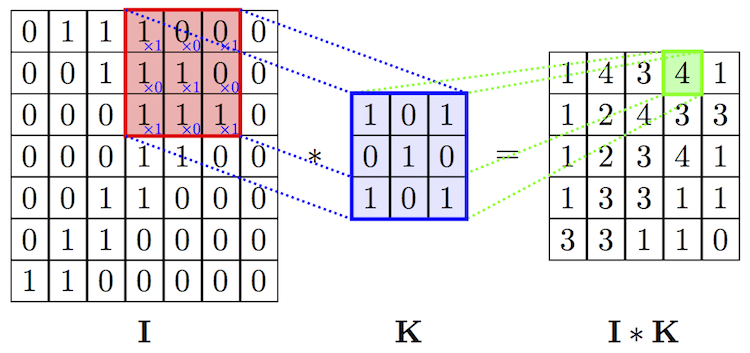
\includegraphics[width=0.7\linewidth]{An-example-of-convolution-operation-in-2D-2.png}
    \caption{2D convolution - Scientific Figure on ResearchGate. Available from: \url{https://www.researchgate.net/figure/An-example-of-convolution-operation-in-2D-2_fig3_324165524} [accessed 31 Mar, 2020]}
    \label{fig:2d-conv}
\end{figure}

\vspace{4mm}

\par There are two main branches of machine learning, such as supervised and unsupervised learning. In applications of computer vision supervised learning is used most of the time. These are methods for image classification, object detection/segmentation. These all work by defining an objective function we want to minimize to achieve a desired rate of error. 

\subsubsection{Binary classification}

\par The simplest case is probably binary classification. In binary classification we want to maximize the joint probability of getting a data point $x$ and by applying a function $f(x, \theta) = \hat{y}$, where $\theta$ are function parameters, we predict $\hat{y}$ probability for $x$ being in class $1$ and therefore $1 - \hat{y}$ probability for being in class $0$. If $y$ is the true label of the data point, then we can formalize our explanation as:

\vspace{4mm}

\begin{align}
    P(y = 1 | x) = \hat{y} \\
    P(y = 0 | x) = 1 - \hat{y} \\
    \quad \rightarrow P(y | x) = \hat{y}^{y} \cdot (1 - \hat{y})^{(1-y)}
\end{align}

\vspace{4mm}

\par We want to maximize the sum of this joint probability for all the examples we have in a dataset but we can do so by taking the logarithm of this since the logarithm function is bijective. We call this our objective or loss function we aim to minimize:

\vspace{4mm}

\begin{equation}
    L\big(y, \hat{y}\big) = -\sum_{i = 1}^{N_{data}} \Big(y^{(i)}\log\hat{y}^{(i)} + (1 - y^{(i)})\log(1 - \hat{y}^{(i)})\Big)
\end{equation}

\vspace{4mm}

\par As we acquired $\hat{y}^{(i)}$ by a function $f(x^{(i)}, \theta) = \hat{y}^{(i)}$ on the data point $x$ with parameters $\theta$ therefore the objective function is parametrized by $\theta$ as well. So by feeding exemplary data points to $f$ and calculating the loss we could also calculate the corresponding derivatives of the loss to the parameters $\frac{\partial L}{\partial \theta}$ and apply these derivatives with a predefined rate $\mu$ to improve the objective. We call this gradient descent since the gradient of the function gives the biggest slope on the multidimensional surface spanned by $\theta$ and if we move to the opposite direction of the gradients we then minimize the desired function. We call it batch stochastic gradient descent (SGD) if only a batch of samples is used due to computational resource limitations. This introduces noise to the learning process but if we sample the data uniformly we could still improve the objective function in many iterations:

\vspace{4mm}

\begin{equation}
    L_{batch} = - \sum_{\#batch\_size}L(y^{(i)}, \hat{y}^{(i)}) = L_{batch}(\theta)  
\end{equation}

\vspace{4mm}

\par The gradient with respect to (w.r.t) $\theta$ can be applied with batch SGD in the update step after each sample of data points:

\vspace{4mm}

\begin{equation}
    \theta = \theta - \mu \frac{\partial L}{\partial \theta}
\end{equation}

\vspace{4mm}

\par As it is evident from above any type of differentiable objective function can be used with any differentiable model $f$ and the model can be trained on samples of the dataset to yield a successful predictor for previously unseen data points. Computer vision aims to be able to generalize algorithms as much as possible. The success of deep learning and convolutional neural networks lies in generalization since with large enough datasets they have a very close performance on unseen data as on training data. Therefore we could train a model to recognize lung damage on CT scans on a large enough dataset and apply it in every hospital in the world where they have a gaming graphics card. This solution is feasible and can improve healthcare tremendously. For lower-risk applications, it is even possible to run models in the browser using WebGL technology that recognizes the graphics capabilities of the underlying machine and uses it to run trained models \cite{cohen2019chester}.

\vspace{4mm}

\subsubsection{Structure of a CNN}

\par The structure of a convolutional neural network is the following: the input is a 3-dimensional array, representing an image. The image is then fed-forward through convolutional layers with different sized and number of filters. The main intuition behind selecting the right filter/kernel sizes comes from the VGG16 architecture \cite{simonyan2014very}. The main intuition is that small kernels, usually $3x3$, can have a high receptive field after many layers, therefore using larger kernels only uses more computational resources and is not that useful. Since the image is compressed after some or each convolution by maximum or average pooling or strided convolutions it is usually so that the number of kernels used is increased with the spatial size decreased. After convolutional layers, the data is flattened into a vector and fed to a multi-layer perceptron which is matrix multiplications followed by non-linearities.

\vspace{4mm}

\begin{figure}[H]
    \centering
    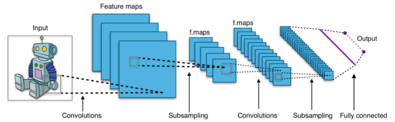
\includegraphics[width=.8\linewidth]{wiki_cnn.png}
    \caption{Structure of a convolutional neural network - Convolutional neural networks, Wikipedia}
    \label{fig:my_label}
\end{figure}

\vspace{4mm}

\par The non-linearities or activation functions are applied after each layer to make the computation non-linear. This is necessary since a linear computation can always be represented by matrix multiplication. The best working non-linearity proved to be the rectified linear unit ReLU in deep learning and is used throughout networks. The last non-linearity, on the other hand, can be different based on the problem. For regression, it might not be needed with unbounded predictions, for binary classification the sigmoid function is used which saturates the real number in a (0, 1) interval and for non-binary classification the softmax function is used which return a probability distribution among N classes for each sample.

\vspace{4mm}

\begin{minipage}[t]{0.45\textwidth}
    \centering
    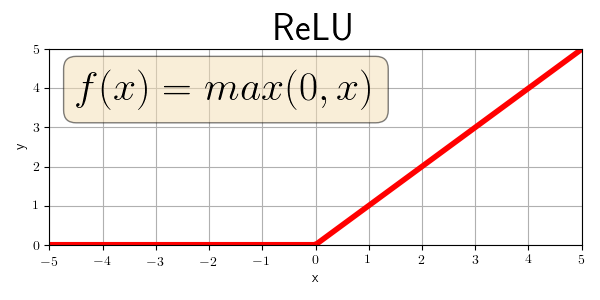
\includegraphics[width=\textwidth]{relu.png}
    \captionof{figure}{Rectified linear unit}
    \label{fig:relu}
\end{minipage}
\begin{minipage}[t]{0.45\textwidth}
    \centering
    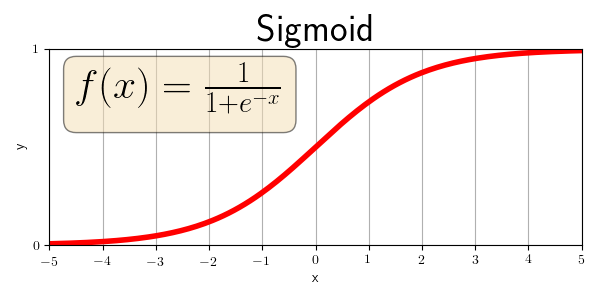
\includegraphics[width=\textwidth]{sigmoid.png}
    \captionof{figure}{Sigmoid}
    \label{fig:sigmoid}
\end{minipage}

\vspace{4mm}

\begin{equation}
    softmax(\vec{x}) = \frac{e^{\vec{x}}}{\sum_{i}e^{\vec{x}_i}}
\end{equation}

\vspace{4mm}

\par We have seen the objective function for binary classification before where we use the sigmoid activation function to acquire probabilities from the model but in the case of multi-class labels we use the cross-entropy loss that is defined as:

\vspace{4mm}

\begin{equation}
    L_{CE} = - \sum_{i = 1}^{N_{class}} y_{i}\log\hat{y_{i}}
\end{equation}

\vspace{4mm}

\par For multi-object detection and segmentation much diverse and more intricate loss functions are used and the networks themselves \cite{ren2015faster} are modified as well to handle sliding-windows efficiently via convolutions \cite{redmon2016you}.

\vspace{7mm}

\section{Medical imaging}

\vspace{7mm}

\par Medical imaging was a thing since the discovery of the X-ray. In the beginning, as in photography, they used light sensitive materials to capture the different amount of radiance from the light source but as everything became digitized in the 20th century the field moved on to using silicon-based sensors. These capture data that can be converted to pixel values and used by the computer. Some kind of image processing is inevitable due to contrast, brightness, hue and other corrections such as image stabilization for moving objects.

\vspace{4mm}

\par In medicine and biology a fast digitization process can be experienced. Even in Hungary clinics are starting to realize that the future is based on digital processing of biological samples. There are some techniques that were inherently digital such as MRI \footnote{magnetic resonance imaging} and fMRI \footnote{functional-MRI} and PET \footnote{positron emission tomography} due to the process involved requiring the image, however, in pathology were a large amount of biopsies are taken each year the case is not so. Medics usually scan to manually sliced slices of tissue via optical microscopes and make decisions based on that. This methods works well and is reliable but does not scale well. 

\vspace{4mm}

\par There exist many companies that manufacture digital microscopes that can process many slides of tissue samples a day and save the high-quality images to a local, clinical database. With the advent of deep learning this data can be pre-processed via computer vision algorithms. It is only a matter of proper data acquisition by the clinical institutes to enable large scale applications such as automatized negative case dismissal, cell count in any kind of tissue, alerts on maligns cases and even improved diagnostic capabilities.

\vspace{7mm}

\subsection{Cancer detection}

\vspace{7mm}

\par Reading mammograms and evaluating tissue samples for colorectal cancer takes years of practice after acquiring a degree in medicine. The skill is gathered by seeing many samples and noticing little but usual similarities between different patients. 

\vspace{4mm}

\par For mammography the image is an X-ray scan of the tissue and noticing nodules is the goal. In Hungary and also in the UK it is mandatory for a medic after finishing university to obtain a certificate for reading mammograms since it is not a trivial thing to do well. On the other hand, there are countries where this is not required and it shows in performance, which is shown in \cite{mckinney2020international}.

\vspace{4mm}

\par For pathologist the tissue is usually stained with H\&E \footnote{haemotoxylin and eosin} staining, which is a standard protocol \cite{fischer2008hematoxylin}, that has a specific purple and pink color. Inspecting these through microscopes enables doctors to issue diagnosis based on the visual attributes of the samples.

\vspace{4mm}

\par Since it seems that cancer detection in such tissue is mainly based on visual attributes of the environment it should not be surprising that the task can be done with convolutional neural networks.

\vspace{4mm}

\par According to the WHO \footnote{World Health Organization} every one death out of six is due to cancer \cite{whoCANCER}. The leading cancer type among women is breast cancer while it is colorectal cancer in men. We disregard here the large case number of lung cancer since it is mainly due to smoking and is in decay for decades now.

\vspace{4mm}

\begin{figure}[H]
    \centering
    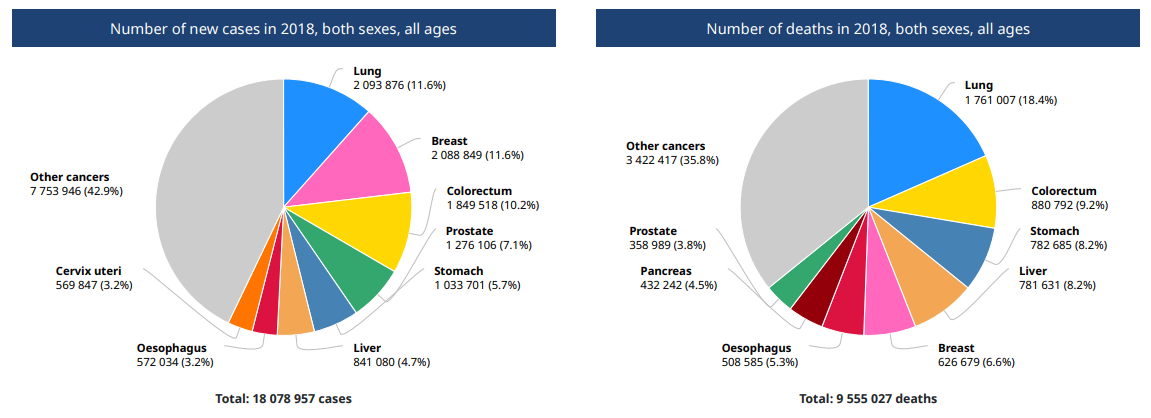
\includegraphics[width=0.8\textwidth]{all_cancer_pie_charts.png}
    \caption{New cancer cases and death rates according to the International Agency on Cancer Research,  WHO}
    \label{fig:cancer_pie_chart}
\end{figure}

\vspace{4mm}

\par The lower than expected death rate in breast cancer is due to the national screening programs that are able to detect malign lesions before they are in a terminal state. National colorectal cancer screening programs have been launched in the past decade in the Netherlands \cite{rivm_2014}, in the UK \cite{gov.uk_2015} and is rolling out or in an early stage in many other countries according to the European Union \cite{euReportOnCancer}.

\vspace{4mm}

\par A national screening program requires a lot of effort from pathologist and much more highly-skilled working hours that is available in any country. It cannot be a short-term solution to educate more doctors in this skill for obvious reasons, therefore we should turn to other available solutions. One is to automate as many things as possible. For screening programs a huge impact can be achieved by dismissing negative samples and only letting through positive ones with extremely high precision and crucially low false-negative rate. On the other hand, one might be interested in pre-selecting high-risk patients based on the diagnosis to start treatment as soon as possible.

\newpage

\section{Deep learning in pathology}

\vspace{7mm}

\par In the project we have been working on in collaboration with the 2nd Department of Pathology- Semmelweis University we aimed to collect a large amount of digitized whole slide scans from rectal biopsies and annotate them with expert pathologist. The annotation process included global labels and local, free-hand area annotations for specific lesions. Having acquired the necessary amount of data we developed and validated a sophisticated autonomous detection system via computer vision techniques. We qualitatively compare the AI pathologist with human experts in all categories.

\vspace{4mm}

\subsection{Screening process}

\vspace{4mm}

\par The screening process involves the following steps: first a surgeon takes a sample from the bowel of the patient and he/she sends it to histology where pathologist analyze and diagnose the sample. We use these digitized samples to make a diagnoses with the autonomous system.

\vspace{4mm}

\subsection{Similar studies}

\vspace{4mm}

\par Many studies have emerged in the past few years using modern computer vision techniques in biomedical imaging and bowel tissue analysis is not an exception at all. One of the first studies occupied with rectal polyp classification \cite{korbar2017deep}, while an other study extract features with a deep network trained on natural images and uses those features to predict a more precise grade for the COAD WSI \footnote{Colon Adenocarcinoma Whole Slide Imaging} data \cite{bychkov2018deep}. A recent study similar to ours shows \cite{skrede2020deep} survival probability based on whole slide images.

\vspace{4mm}

\subsection{Goals}

\vspace{4mm}

\par There are a few distinct ways of handling large scale whole slide images. Usually in deep learning images are sized less than \begin{markdown}
`1024 x 1024 x 3`
\end{markdown} 
pixels and therefore one can cut out small pieces of a large image and train a network on that data to classify the patches, this was done by \cite{korbar2017deep}, \cite{bychkov2018deep} and \cite{skrede2020deep}. It is also possible to extract features from these smaller patches and then put together those as training data for a new network to classify the whole image in its integrity for something, this was done by \cite{skrede2020deep} and we have a very similar approach but not for survival but total whole slide patch level segmentation of the image. We aim to categorize every patch and draw a diagnosis based on the full slide. In order to make our diagnoses interpretable we need to categorize every region as a human would do and give back localized information and reduce that to a diagnoses later on. Our work is also very similar to \cite{takahama2019multi} since we use a two step prediction process in order to acquire higher accuracy.

\vspace{4mm}

\subsection{Data}

\vspace{4mm}

\par The tissue segments were scanned at 400x zoom and annotated with the QuPath v0.1.2. software. The software included a viewer and a free-hand ROI \footnote{region of interest} annotator tool but I needed to write a plugin in order to extract the annotation data. This open-source plugin was developed in Java and is available at \url{https://github.com/qbeer/qupath-binarymask-extension}. Basically the extension is capable of extracting and loading annotation masks from a pre-specified directory into a QuPath project. The annotation mask are saved into PNG format in black and white for efficient storing and in reduced size based due to very annotated regions.

\vspace{7mm}

\begin{minipage}[t]{0.4\textwidth}
    \centering
    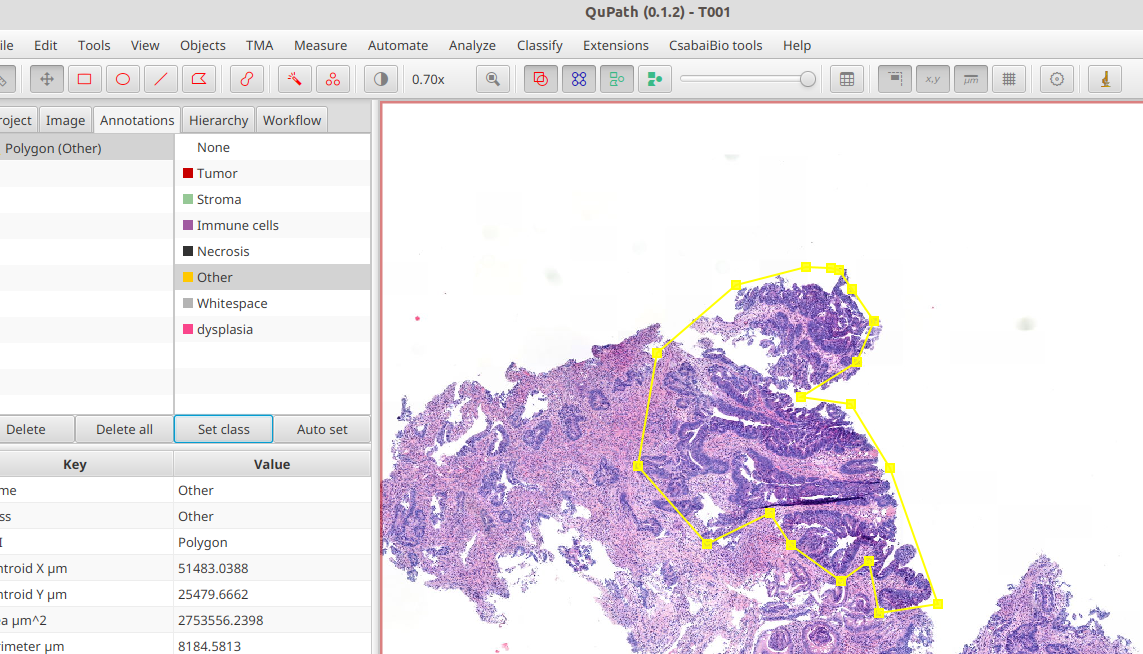
\includegraphics[width=\linewidth]{qupath_screenshot.png}
    \captionof{figure}{View of the annotated region in QuPath, all the metadata saved in the filename of the annotation}
    \label{fig:annotation_qupath}
\end{minipage}\qquad\qquad
\begin{minipage}[t]{0.4\textwidth}
    \centering
    
\includegraphics[width=.5\linewidth]{T001_Other_(4.00,416425,200638,17047,19660)-mask.png}
    \captionof{figure}{(package, annotation type, down-scaling factor, x, y, width, height) : T001\_Other\_(4.00,416425,
    200638,17047,19660)-mask.png}
    \label{fig:annotation}
\end{minipage}

\vspace{7mm}

\par After this the images were processed via Python. We cut out \begin{markdown} 
`512 x 512 x 3`  
\end{markdown} 
sized patches and matched the location of the annotations to the corresponding patches therefore getting patch level segmentation of the whole slide image. In order to get rid of the meaningless patches, those that were mainly white, containing only tissue residue or scanning errors we applied pixel thresholds on the patches. We took the intensity from the HSI components (hue, saturation and intensity) and set a threshold of 245 for 8 bit pixels to extract all the white patches. We also calculated the saturation for the patch and if it was less then .05 we said that the pixel is mainly gray, therefore useless and excluded it.

\begin{figure}[H]
    \centering
    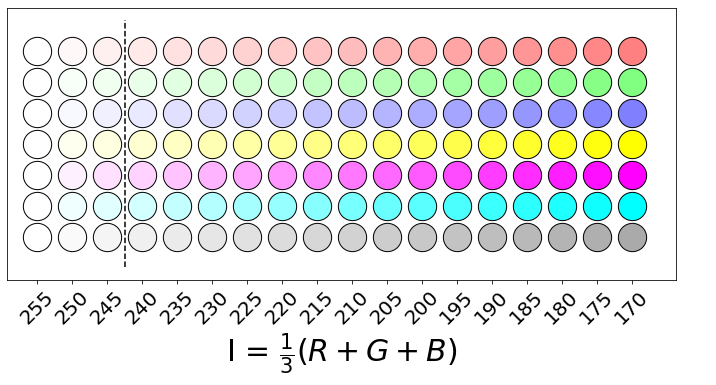
\includegraphics[width=.6\textwidth]{intensity.png}
    \caption{White limit}
    \label{fig:intensity}
\end{figure}

\begin{figure}[H]
    \centering
    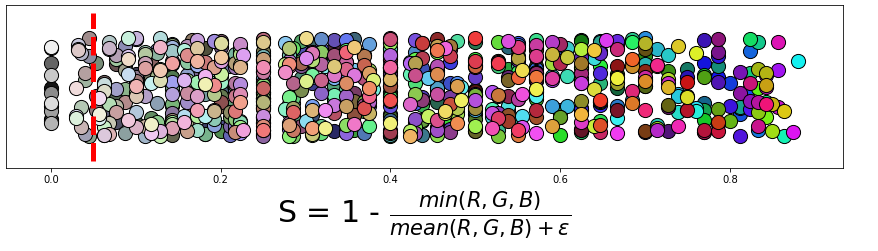
\includegraphics[width=.7\textwidth]{saturation.png}
    \captionof{figure}{Gray limit}
    \label{fig:saturation}
\end{figure}

\vspace{4mm}

\par Here I also provide an illustration to justify this and show the image patches acquired as a result after applying this thresholding methodology. It is obvious that the method took care of removing the residual tissue and remains of grime (dirt particles, fur, hair, etc.) on the glass plate that the slide was on.

\vspace{10mm}

\begin{minipage}[t]{0.45\textwidth}
    \centering
    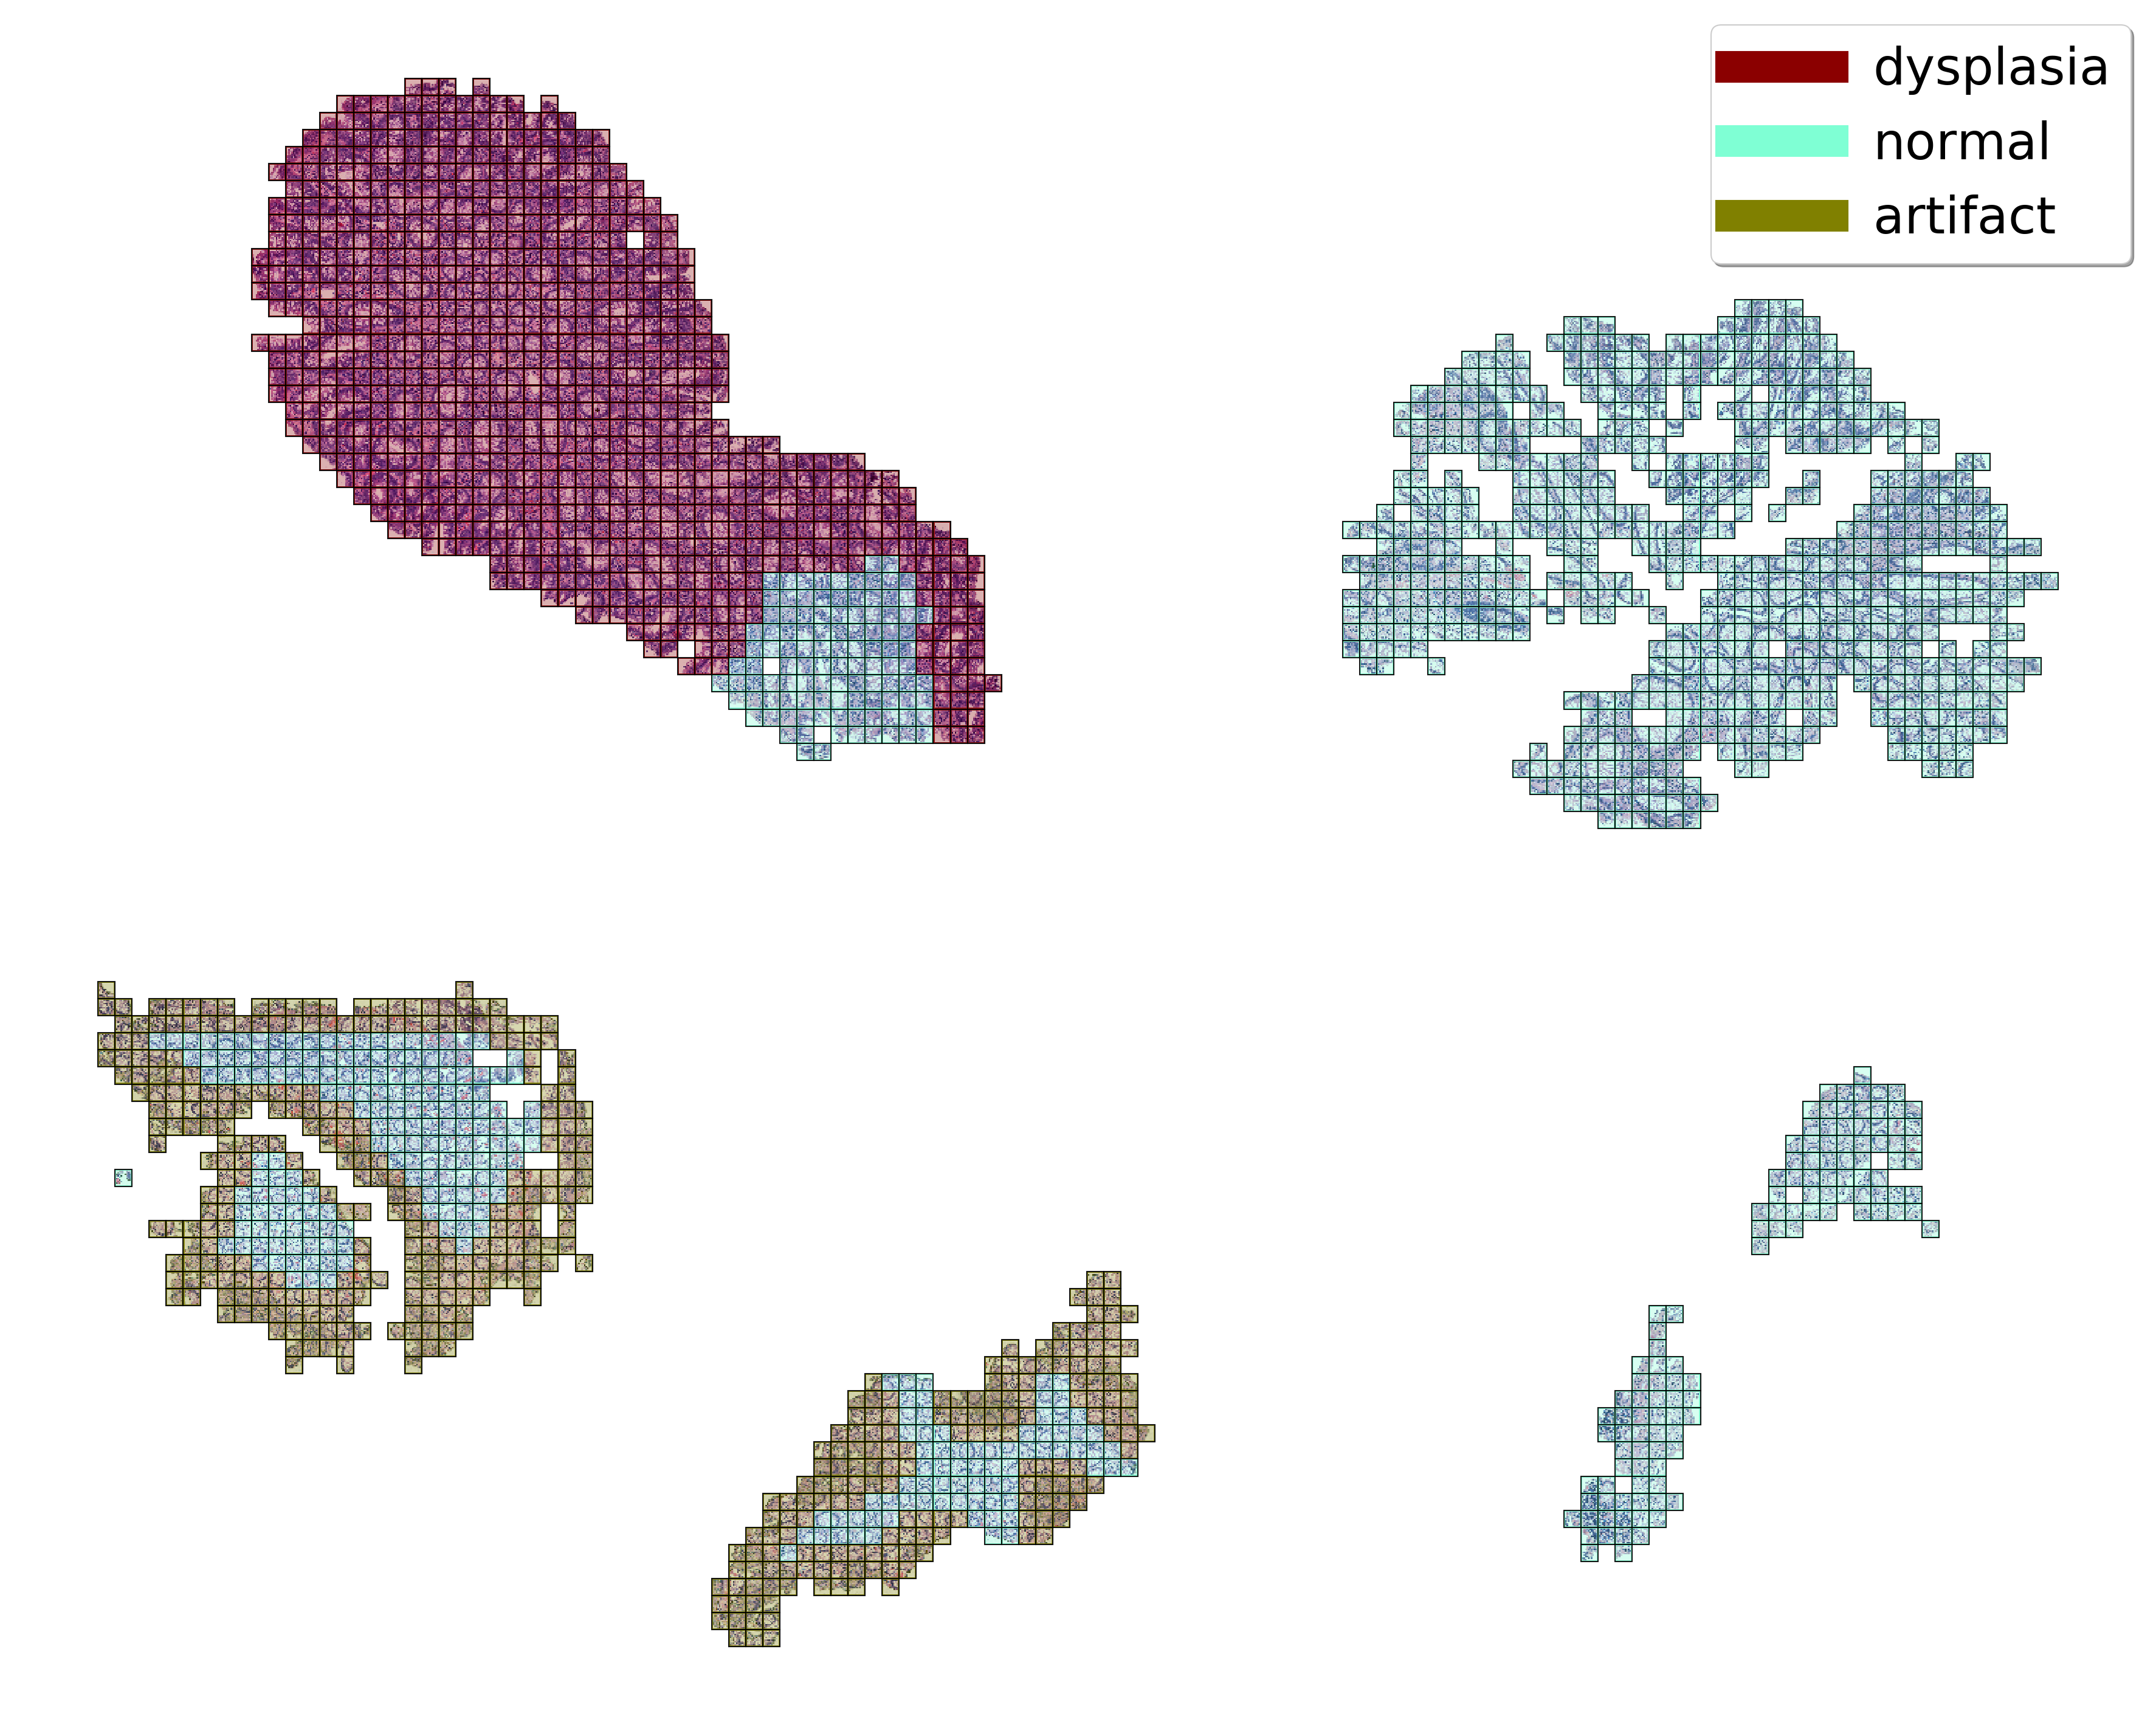
\includegraphics[width=\textwidth]{082_19_16683_zoom_1.15.png}
    \captionof{figure}{Image after thresholding and patching - with the corresponding masks on top}
    \label{fig:preprocessedslide}
\end{minipage} \qquad
\begin{minipage}[t]{0.45\textwidth}
    \centering
    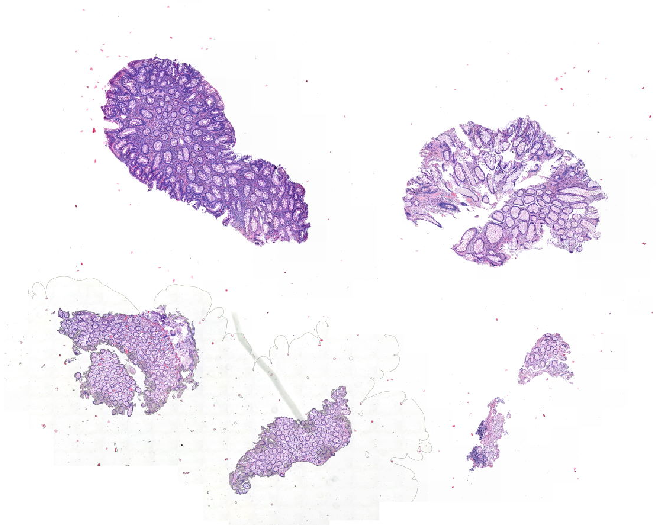
\includegraphics[width=\textwidth]{082_qupath.png}
    \captionof{figure}{The original image before the pre-processing}
    \label{fig:origslide}
\end{minipage}

\vspace{7mm}

\par The prediction process happens in two stages, the first is a patch-level classification that will be detailed later. The second process is a modified U-Net \cite{ronneberger2015u} architecture that we applied to predict a semantic segmentation map of the WSI in lower resolution. The input was a down-scaled version of the original whole slide image and each pixel was an intermediate feature from the classifier, therefore, the input contained many more channels than the usual R, G, B color channels. This had to be stored in a separate dataset and needed to be rebuilt for each and every classifier that we trained.

\vspace{4mm}

\subsubsection{Data for testing}

\vspace{4mm}

\par The test dataset was annotated by board certified, expert pathologists. They annotated the slides without any additional information and got the images anonymized. They needed to record all local and global categories in check boxes to draw clinical conclusion and we ignored free-hand annotation as it was not crucial for comparison in clinical diagnosis. 

\vspace{4mm}

\subsubsection{Annotation categories}

\vspace{4mm}

\par We gathered two main types of annotations for the dataset: local and global labels. Locally we asked pathologists to annotate the following regions by drawing free-hand masks on the slide with QuPath. The categories were selected based on clinical relevance, expert review and consensus.

\vspace{4mm}

\begin{enumerate}
    \item \textbf{dysplasia} - abnormal epithelial growth
    \item \textbf{highgrade\_dysplasia} - severe dysplasia (annotated inside dysplasia)
    
    \begin{minipage}[t]{0.45\textwidth}
        \centering
        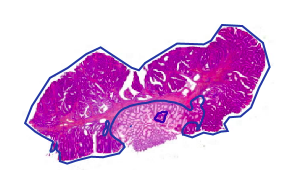
\includegraphics[width=.8\linewidth]{dysplasia.png}
        \captionof{figure}{Dysplasia}
    \end{minipage}
    \begin{minipage}[t]{0.45\textwidth}
        \centering
        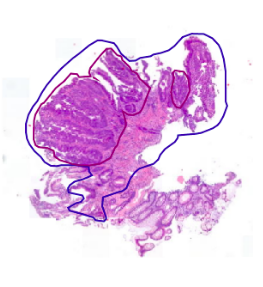
\includegraphics[width=.8\linewidth]{high_grade_dysplasia.png}
        \captionof{figure}{High-grade dysplasia}
    \end{minipage}
    
    \item \textbf{adenocarcinoma}
    \item \textbf{suspicious\_for\_invasion} - obvious signs of invasion
    \item \textbf{inflammation}
    \item \textbf{resection\_edge}
    \item \textbf{tumor\_necrosis}
    \item \textbf{lymphovascular\_invasion}
    \item \textbf{artifact}
    \item \textbf{annotated} - there are several slides present on one scan and one should be randomly selected and annotated
    
    \begin{figure}[H]
        \centering
        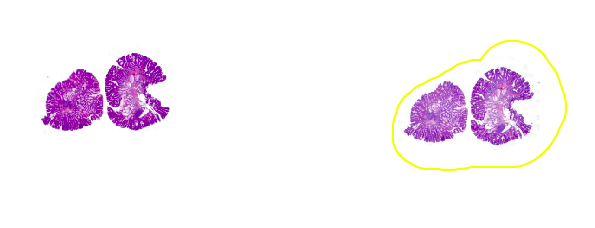
\includegraphics[width=0.6\textwidth]{annotated.png}
    \end{figure}
    
\end{enumerate}

\par Above some illustration is present with the annotated local categories. For the global labels the below list was selected:

\vspace{4mm}

\begin{itemize}
    \item main\_category
    \begin{itemize}
        \item CRC - colorectal cancer
        \item advanced\_adenoma
        \item non\_neoplastic\_leison
        \item negative
    \end{itemize}
    \item Haggit\_level \cite{aarons2014management}
    \item polyp\_type
    \begin{itemize}
        \item hyperplastic\_polyp
        \item sessile\_serrated\_polyp
        \item traditional\_serrated\_adenoma
        \item tubular\_adenoma
        \item tubulovillous\_adenoma
        \item villous\_adenoma
        \iteme hybrid
    \end{itemize}
    \item biopsy\_or\_polyp - (either biopsy or polyp, the type of the sample)
    \item other comments
\end{itemize}

\vspace{4mm}

\subsection{Vision models}

\vspace{7mm}

\par Our vision models were implemented in Tensorflow v2.0. and as I mentioned before it was a two step process. The first model was a ResNet50 based architecture \cite{he2016deep} with a fully-connected head on top of it. Optimization was done with the Rectified Adam optimizer \cite{liu2019variance} with lookahead \cite{zhang2019lookahead}. The objective function was the sum of pairwise binary cross-entropy loss since a patch could be labeled with more categories if its on a mask edge. This model has approximately 24 million trainable parameters: 

\vspace{4mm}

\begin{table}[H]
    \centering
    \begingroup
    \setlength{\arrayrulewidth}{0.1mm}
    \setlength{\tabcolsep}{22pt}
    \renewcommand{\arraystretch}{1.7}
    \scriptsize
    \begin{tabular}{| c | c |} \hline
        \textbf{layer} name &  \textbf{ResNet50} \\ \hline
        conv1 &  7 \times 7, 64, stride 2 \\ \hline
        conv2\_x &  \makecell{3 \times 3 \quad max \quad pool, \quad stride \quad 2 \\ \begin{bmatrix}
1 \times 1, 64 \\
3 \times 3, 64 \\
1 \times 1, 256 
\end{bmatrix} \times \quad 3} \\ \hline
        conv3\_x &  \makecell{ \begin{bmatrix}
1 \times 1, 128 \\
3 \times 3, 128 \\
1 \times 1, 512 
\end{bmatrix} \times \quad 4} \\ \hline
        conv4\_x &  \makecell{ \begin{bmatrix}
1 \times 1, 256 \\
3 \times 3, 256 \\
1 \times 1, 1024 
\end{bmatrix} \times \quad 6} \\ \hline
        conv5\_x & \makecell{ \begin{bmatrix}
1 \times 1, 512 \\
3 \times 3, 512 \\
1 \times 1, 2048 
\end{bmatrix} \times \quad 3 } \\ \hline
        & average pool, 256-d fc, 128-d fc, 10-d fc \\ \hline
    \end{tabular}
    \endgroup
    \caption{Caption}
    \label{tab:my_label}
\end{table}

\vspace{4mm}

\par We applied binary cross-entropy loss between all pairs, the parameters were $10^{-4}$ base learning rate for the Rectified Adam optmizer which decayed in $45'000$ steps to $5 \cdot 10^{-6}$ while the lookahead optmizer did updates with a $0.5$ step size after six steps of exploration.

\newpage

\bibliographystyle{unsrt}
\bibliography{references}

\end{document}\grid
